% !TEX encoding = UTF-8 Unicode
% !TEX program = pdflatex
% !TEX spellcheck = en_US

\documentclass[amsthm,ebook]{saparticle}

% IF YOU USE PDFLATEX
\usepackage[utf8x]{inputenc}
% if you write in english and in greek
\usepackage{ucs}
\usepackage[greek,english]{babel}
\usepackage{float}
\usepackage[table]{xcolor}
\languageattribute{greek}{polutoniko}

% IF YOU USE XELATEX
%\usepackage{polyglossia}
% if you write in italian
%\setmainlanguage{italian}
% If you want put some ancient greek:
%\setotherlanguage[variant=polytonic]{greek}
%\newfontfamily{\greekfont}[Ligatures=TeX]{Palatino Linotype}

% dummy text (remove in a normal thesis)
% remove if not necessary
%\usepackage{siunitx}
%Natbib for bibliography management
\usepackage[authoryear]{natbib}
% custom commands
\newcommand{\bs}{\textbackslash}

%%%%%%%%
%TITLE:%
%%%%%%%%
\title{The EAGLE Data Aggregator:
Data Quality Monitoring}

%%%%%%%%
%AUTHORS:%
%%%%%%%%
\author[CNR-ISTI]{Andrea Mannocci\corref{all}}
\author[CNR-ISTI]{Vittore Casarosa\corref{all}}
\author[CNR-ISTI]{Paolo Manghi\corref{all}}
\author[CNR-ISTI]{Franco Zoppi\corref{all}}

%Additional information about corresponding author, addresses and affiliations:
\cortext[all]{Corresponding authors: \{andrea.mannocci, vittore.casarosa, paolo.manghi, franco.zoppi\}@isti.cnr.it
}

\address[CNR-ISTI]{ISTI - Area della Ricerca CNR, via G. Moruzzi 1, 56124 Pisa, Italy}

%%%%%%%%%%%%
%PAPER CONTENT %
%start your paper here%
%%%%%%%%%%%%
\begin{document}
\rowcolors{2}{gray!25}{white}
\maketitle

\begin{abstract}
The EAGLE project aggregates epigraphy related content from about 20 different data providers, and makes its content available to both Europeana and to scholars. Data Quality monitoring is a key issue in Aggregative Data Infrastructures, where content is collected from a number of different sources with different data models and quality standards. This paper presents a Monitoring Framework for enabling the observation and monitoring of an aggregative infrastructure focusing on the description of the Data Flow and Dynamics Service, and exemplifying these concepts with a use case tailored to the characteristics of the EAGLE aggregation data flow.

An Infrastructure Quality Manager (IQM) is provided with a Web user interface (WebUI), allowing her to describe the data flows taking place in the infrastructure and to define monitoring scenarios. The scenarios will include the definition of sensors (pieces of software plugged into the data flow), which will provide observations of measured objects. The scenarios include also the definition of controls and analysers, which will store and process the observations received from the sensors and will verify if the values of the measured features comply with some expected behaviour over time. 

A monitoring scenario for EAGLE has been defined and tested on simulated data (the monitoring framework is still under development) in order to monitor the ``health'' of different data collections involved in the EAGLE collection and transformation workflows.  

\end{abstract}

\keywords{EAGLE, Aggregative Data Infrastructure, Data Quality, Metrics, Monitoring.}

\section{Monitoring framework}\label{framework}

The EAGLE project \citep[fully described in][]{eagle} aggregates epigraphy related content from about 20 different data providers (cultural institutions all over Europe), and makes its content available to both Europeana \citep{europeana} (through an OAI-PMH interface) and to scholars and the general public through a Web portal.

Collecting data provided by a number of different sources, very often with different quality standards, presents the challenge of measuring the overall quality of the aggregated data, and how it compares with standards and objectives set by the aggregating institution.

We present here an extension to EAGLE that will take advantage of a \textit{Monitoring Framework} (being developed in the context of another project \citep{openaire}), enabling the observation and monitoring of an Aggregative Data Infrastructure over time. 

By modelling ``data processing'' as a manufacturing process involving data \citep{ballou1998}, the Monitoring Framework provides tools for the automatic extraction of observations (numeric indicators about properties of the system) from the context where the data is being processed and stored, providing time series of indicators expressed in user-defined metrics.

The Monitoring Framework offers a \textit{Data Flow and Dynamics Service} (DFDS for short) to the \textit{Infrastructure Quality Manager} (IQM for short), a role that (hopefully) will become standard in data aggregation infrastructures. The DFDS enables the IQM to create one or more monitoring scenarios, each designed to monitor a particular functional area or aspect of the aggregation infrastructure. For example, an EAGLE monitoring scenario could deal with the workflow that builds the aggregated content to be used by the EAGLE Web portal and by Europeana’s OAI-PMH harvesters \citep{mannocci2014}. After the collection and processing of (possibly heterogeneous) records coming from different content providers, the aggregator stores them into different environments, for different purposes. More precisely: \textit{i)} the processed records are indexed as a full-text index (implemented by Apache Solr) to support search and browse queries from the EAGLE Web portal; \textit{ii)} the processed records are stored also in a document store (implemented by MongoDB) to support OAI-PMH requests. In this case, for example, we might be interested in assessing (and keep assessing over time) whether the total number of artifacts indexed by Solr matches the number of artifacts delivered via OAI-PMH. This could easily be accomplished by monitoring the number of records stored in the index and the number of records stored in the document store, and comparing their values. As another example, we might be interested in verifying whether the trend of a certain property of the monitored system complies with a given criterion (e.g. the number of records per content provider should be strictly increasing over time).

Using the Data Flow and Dynamics Service provided by the Monitoring Framework, it is possible to define \textit{monitoring scenarios}, which define a conceptualization of the data flows taking place in the aggregating infrastructure. Similarly to what happens to goods in a manufacturing process, data collections and processes acting over that data can be observed thanks to specially devised \textit{sensors}, which in our case are pieces of code providing numeric values about features of interest. The monitoring scenario can also define controls to verify if the values of such features comply with some expected behaviour over time.

With the concept of sensor, we refer to a piece of software capable of generating \textit{observations} (a numeric value plus some contextual metadata) about a measured object. \textit{Measured objects} can be of different granularity, e.g. single data units (datum) or data collections stored somewhere by the aggregating infrastructure. Each observation is expressed in just one specific metric, intended to measure a specific feature of a measured object (e.g. the number of publications present in the data collection stored in the Solr index). A sensor can generate observations in more than one metric, each one referring to a different feature of the measured object. 

A sensor can in principle be plugged anywhere in the aggregating infrastructure; with the understanding that the implementation of the sensor and the point of the data flow where it will be placed are the responsibility of the IQM. When the workflows of the aggregating infrastructure are in execution, the sensors will be activated and will produce a stream of observations. The DFDS will separate the stream of observations into different streams, each one related to a specific metric, and will store them as points of time series. In this way, observations can be queried and examined either as charts or tabular data.

The interaction between the IQM and the Monitoring Framework is done through a user friendly user interface (WebUI) provided by the DFDS. In addition to providing easy access to the observation time series, the WebUI provides the facilities to define the overall Monitoring Scenario, which will include the sensors and the \emph{controls}. 

For the purpose of monitoring, the IQM can define \textit{controls}, i.e. checks that can be scheduled to automatically verify the compliance of one or more metrics (and their observations) with a desired (or un-desired) condition. A control uses an \textit{analyser} for the comparison of observation values, such as, for example, values alignment, less or greater than, (strictly) monotonic increasing or decreasing values, threshold guards, thresholded peak or percentage variation, etc. For example, as mentioned before, we might be interested to check if the number of artefacts indexed by Solr is equal to the number of artefacts exported in OAI-PMH records, or if the total number of EAGLE objects provided by a content provider is steadily increasing over time, or, as a further example, if the ``goodness'' of an EAGLE record (the concept of goodness being defined by the IQM and implemented through sensors and controls) remains above a threshold of 0.8. The Data Flow and Dynamics Service offers some analysers out-of-the-box, but also enables the IQM to develop her own custom analysers.

Finally, the Data Flow and Dynamics Service enables the generation of an exhaustive \textit{report} about the defined metrics and controls providing insights, via the WebUI, in a quick glance about key features and potential issues present in the infrastructure. Given a set of controls, the monitoring service also takes care of raising \textit{alerts} and \textit{notifications} informing the IQM about the status of the infrastructure and its operation.


\section{Architecture}\label{arch}

The Monitoring Framework (see Figure 1) is architected as a client-server application, where a core module (imported and used by the code of the aggregating infrastructure) plays the role of \textit{client}. The infrastructure source code needs to be instrumented in order to put sensors in place and produce observations of the measured objects.

The implementation of a sensor provides the logic to produce a measurement; in general, a sensor is devised to probe a specific object type (thus the typing of the measured object is hardcoded), while its configuration can be defined via WebUI and retrieved at runtime (dynamically). Such a design opens up to configurability and extendibility of the sensor’s collection offered by the DFDS, which in any case comes with off-the-shelf implemented sensors.

The \textit{server} component is a stand-alone web application that receives observations from sensors, stores those observations as time series and runs automatically user-defined controls over this corpus of data. The controls present the outcome of their activity as reports, which are made available to the IMQ via the WebUI. There is also an alert and notification service to warn the IMQ about potential anomalies or wrong operation in the aggregating infrastructure.


\section{The EAGLE use case}\label{usecase}

In order to apply the monitoring framework described above to the EAGLE aggregator, we need to define first a monitoring scenario, based on the actual EAGLE data flow, which must include the following. 
\begin{itemize}
\item Sensors to be used in terms of measured objects and metrics implemented (i.e. functions to apply in order to extract observations). Once deployed and running, a sensor dynamically retrieves its defined configuration from the server whenever it is needed. Metrics identified in this test case are reported in Section \ref{sec:metrics}.
\item Controls representing quality checks to be run against measurements obtained with certain metrics. The framework guides the IQM into the definition of a control according to the scenario defined so far. Controls identified in this test case are reported in Section \ref{sec:controls}.
\end{itemize}


\subsection{Metrics}\label{sec:metrics}

A monitoring scenario has been defined and tested on simulated data in order to monitor the ``health'' of different data collections involved in the EAGLE collection and transformation workflows. In particular, a first collection is stored in a full-text index (Apache Solr) serving search queries, and a second one is stored in a document store (MongoDB) serving data for OAI-PMH export.

In this same scenario, we are interested in monitoring also the collection workflow by inspecting every single native XML record flowing into the EAGLE infrastructure from content providers. Some useful metrics identified in EAGLE are described in Table \ref{tab:metrics}.

\begin{table}
{\small
\addtolength{\tabcolsep}{-0.5mm}
\begin{tabular*}{\textwidth}{ l l }
\toprule
Measured property & Metric\\
\midrule
\parbox[t]{0.6\textwidth}{Total \# of content providers joining the EAGLE infrastructure} & Content providers\\
Total \# of languages for translations & Languages\\
Total \# of EAGLE records & Total records\\
\parbox[t]{0.6\textwidth}{Compliance toward the controlled vocabulary for materials. The values of this metric track the percentage of vocabulary-compliant occurrences in the XML field containing the value for ``material'', over the total amount of occurrences of that field. As an example, if the vocabulary defines the entries ``aaa'', ``bbb'', ``ccc'' and the vocabulary-controlled XML field uses ``aaa'' four times, ``bbb'' three times, and ``xxx'' three times, the metric yields 0.7 (i.e. 7 out of 10 occurrences match the vocabulary).} & Voc:material compliance\\
\parbox[t]{0.6\textwidth}{Completeness of every single collected native XML record. The values of this metric track the percentage of non-empty XML fields among 5 user-defined fields (e.g. title, description, object type, date, material.). The value could be 0\%, 20\%, 40\%, 60\%, 80\%, 100\%, depending on how many non-empty values have been found.} & Completeness\\
\bottomrule
\end{tabular*}}
\caption{Metrics implemented in EAGLE.}
\label{tab:metrics}
\end{table}


\subsection{Controls}\label{sec:controls}

Given the metrics described in \ref{sec:metrics}, Table \ref{tab:controls} reports some controls defined over those metrics.

\begin{table}
{\small
\addtolength{\tabcolsep}{-0.5mm}
\begin{tabular*}{\textwidth}{ l l }
\toprule
Metric & Control\\
\midrule
Content providers & \parbox[t]{0.6\textwidth}{Check if the number of content providers indexed in Solr is monotonic increasing over time (considering the three last observations of the metric)}\\
Content providers & \parbox[t]{0.6\textwidth}{Check whether the number of content providers indexed in Solr equals the number of OAI sets present in MongoDB (considering only the last observation of the metric)}\\
Languages & \parbox[t]{0.6\textwidth}{Check if the number of modern languages present in translations indexed in Solr is steadily increasing over time (considering the two last observations of the metric)}\\
Total records & \parbox[t]{0.6\textwidth}{Check whether the total number of EAGLE records (per content provider) is steadily increasing over time (considering only the three last observations)}\\
Voc:material compliance & \parbox[t]{0.6\textwidth}{Check if such indicator, ranging from 0.0 to 1.0, is above 0.9 threshold (considering only the very last observation of the metric)}\\
Completeness & \parbox[t]{0.6\textwidth}{Check if such indicator (actually its rolling average), ranging from 0.0 to 1.0, is above 0.8 threshold (considering only the very last observation of the metric average)}\\
\bottomrule
\end{tabular*}}
\caption{Controls implemented in EAGLE.}
\label{tab:controls}
\end{table}


\subsection{Sample implementation}\label{sample}

Three different sensors have been defined and implemented for this test on EAGLE: two collection sensors (one for Solr and one for MongoDB) and one single-datum sensor for XML record-by-record inspection. Once the three sensors have been placed in the EAGLE workflow implementation and the EAGLE infrastructure is running, they start to produce observations and deliver them to the server component of the monitoring framework.

As an example, we report in figures included in Section \ref{sec:figures} simulated trends of the defined metrics and relative reports (i.e. the evaluation of controls defined over the metrics).

The metric about the ``Total number of content providers'' is reported in Figure \ref{fig:cps}; as expected, the number of content providers indexed is monotonically (each value is greater or equal to the previous one) increasing, as stated in the leftmost report, and the number of OAI sets present in the data collection stored in MongoDB equals the number of content providers indexed in Solr, as stated in the rightmost report. It is also interesting to notice how the two trends diverged in time back in October. In the simulated data we introduced an \textit{ad-hoc} problem in October, related to the publication of EAGLE records into the OAI-PMH store, which the monitoring service succeeded to discover.

In Figure \ref{fig:lang}, we report the ``Languages'' metric; as expected its trend is strictly increasing over time indicating that the corpus of translations is expanding and that they are correctly integrated into the system.

Figure \ref{fig:tot} shows the total number of EAGLE records for four content providers (CP1, CP2, CP3, CP4) and informs the IQM that everything behaves as expected; in fact, the four reports states that the trends of the metric are always increasing over time.

In Figure \ref{fig:voc}, the metric ``Voc:material compliance'' is depicted. The four trends show that the four content providers (CP1, CP2, CP3, CP4) are in general increasing the quality of their data by enforcing the use of correct values offered by the controlled vocabulary for materials. However, CP1 (in orange), with a 0.83 score, does not meet the threshold requirement (set to 0.9) indicated in the control, thus its report is marked in red notifying the issue.

Figure \ref{fig:comp} reports the oscillations of the record-by-record metric ``Completeness'' (narrowed down to a hundred records sample), while Figure \ref{fig:ravg} reports the associated ``rolling average'' (i.e. each point is the updated average up to that instant). Again, as the last observation of metrics is equal to 0.52, the relative reports is marked in red, as the 0.8 threshold defined in the control is not met.


\section{Conclusions and future work}\label{sec:conclusions}

We have presented here the possible application of the Monitoring Framework concepts to the EAGLE aggregating infrastructure. The Monitoring Framework is ``work in progress'' in another European project related to research data infrastructures \citep{openaire}.

The results presented here are based on simulated data, as the EAGLE infrastructure is not yet instrumented with the sensors needed for collecting observations, but we are planning to instrument it as soon as the development of the Monitoring Framework will reach the \textit{beta} status. 

EAGLE represents an ideal \textit{testbed} for this monitoring technology, as the workflows are clean and well defined, the data collected also is well defined, given the mappings that have been defined between the different incoming records and the EAGLE data model. 

Finally, when EAGLE will be equipped with the final Monitoring Framework, we expect that it will provide valuable data for ensuring that the epigraphy data made available at the EAGLE portal will be of the highest quality. It will also provide valuable feedback to the content providers, helping them to detect possible inconsistencies and lack of information in their data, in order to improve the quality of the data provided to EAGLE and also, even more important, the quality of the data that each content provider makes available to its users.
\clearpage

\section{Figures}\label{sec:figures}
\begin{figure}[H]
\centering
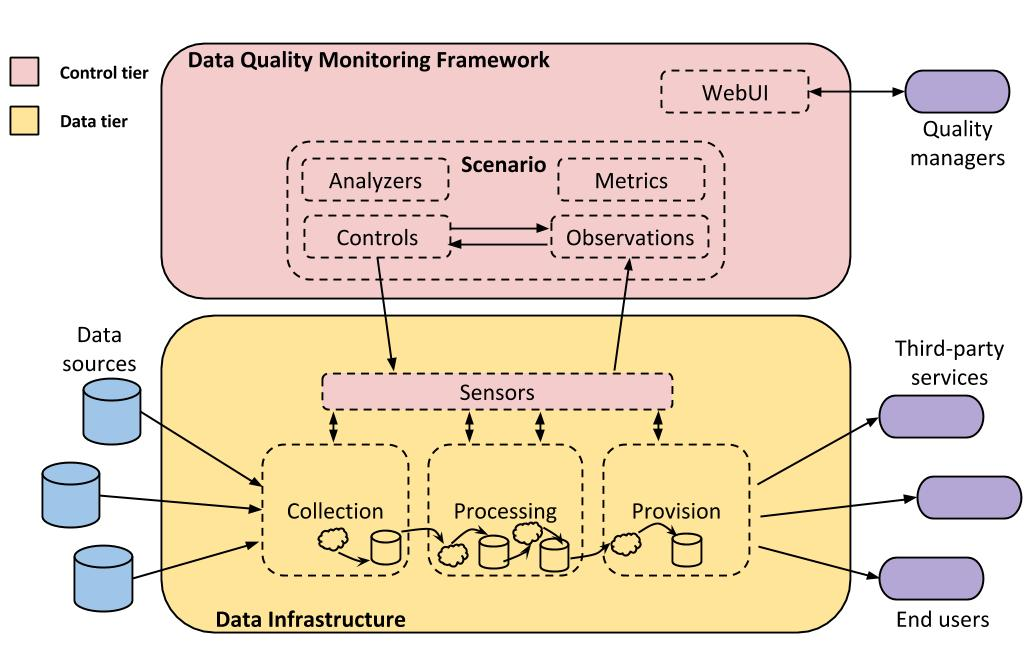
\includegraphics[width=\textwidth]{img/arch.jpg}
\caption{The architectural overview of the monitoring framework.}
\label{fig:arch}
\end{figure}

\begin{figure}[H]
\centering
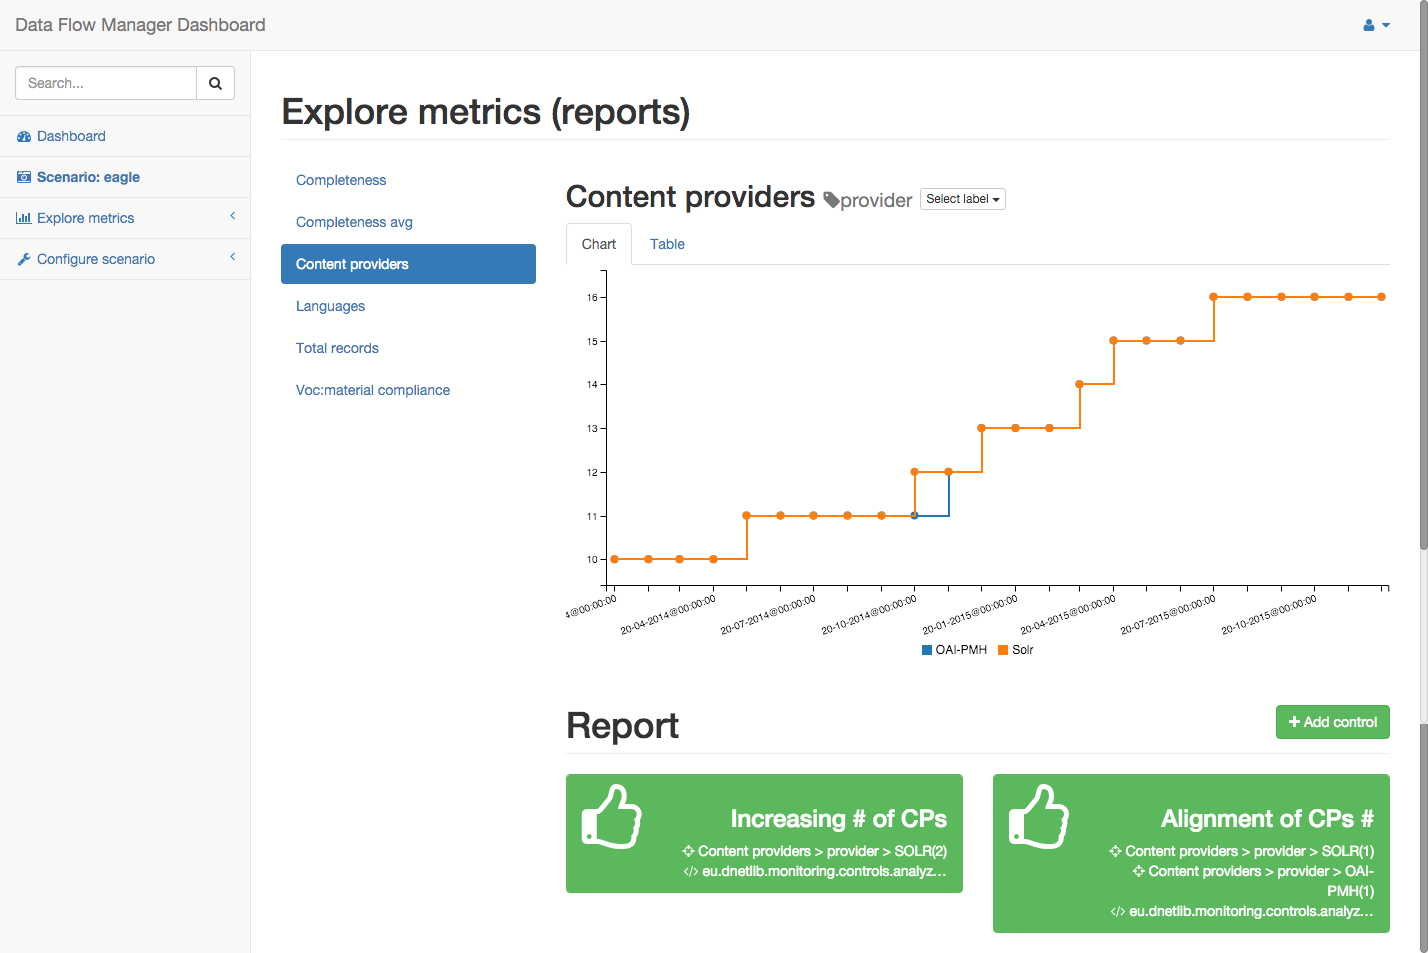
\includegraphics[width=\textwidth]{img/cps.png}
\caption{The trend of the metric ``Total number of content providers''.}
\label{fig:cps}
\end{figure}

\begin{figure}[H]
\centering
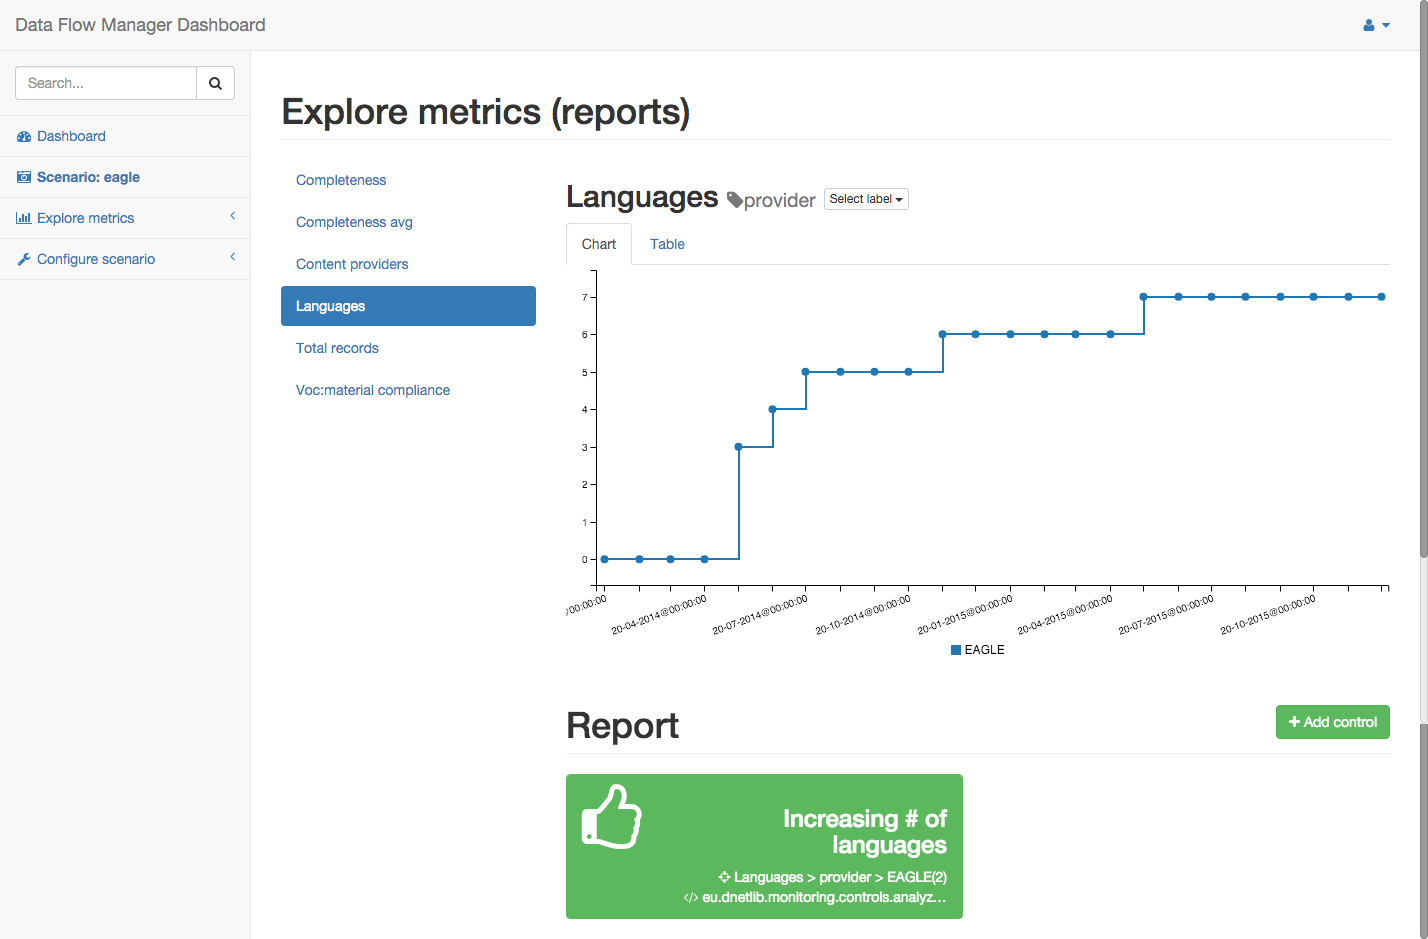
\includegraphics[width=\textwidth]{img/lang.png}
\caption{The trend of the metric ``Languages''.}
\label{fig:lang}
\end{figure}

\begin{figure}[H]
\centering
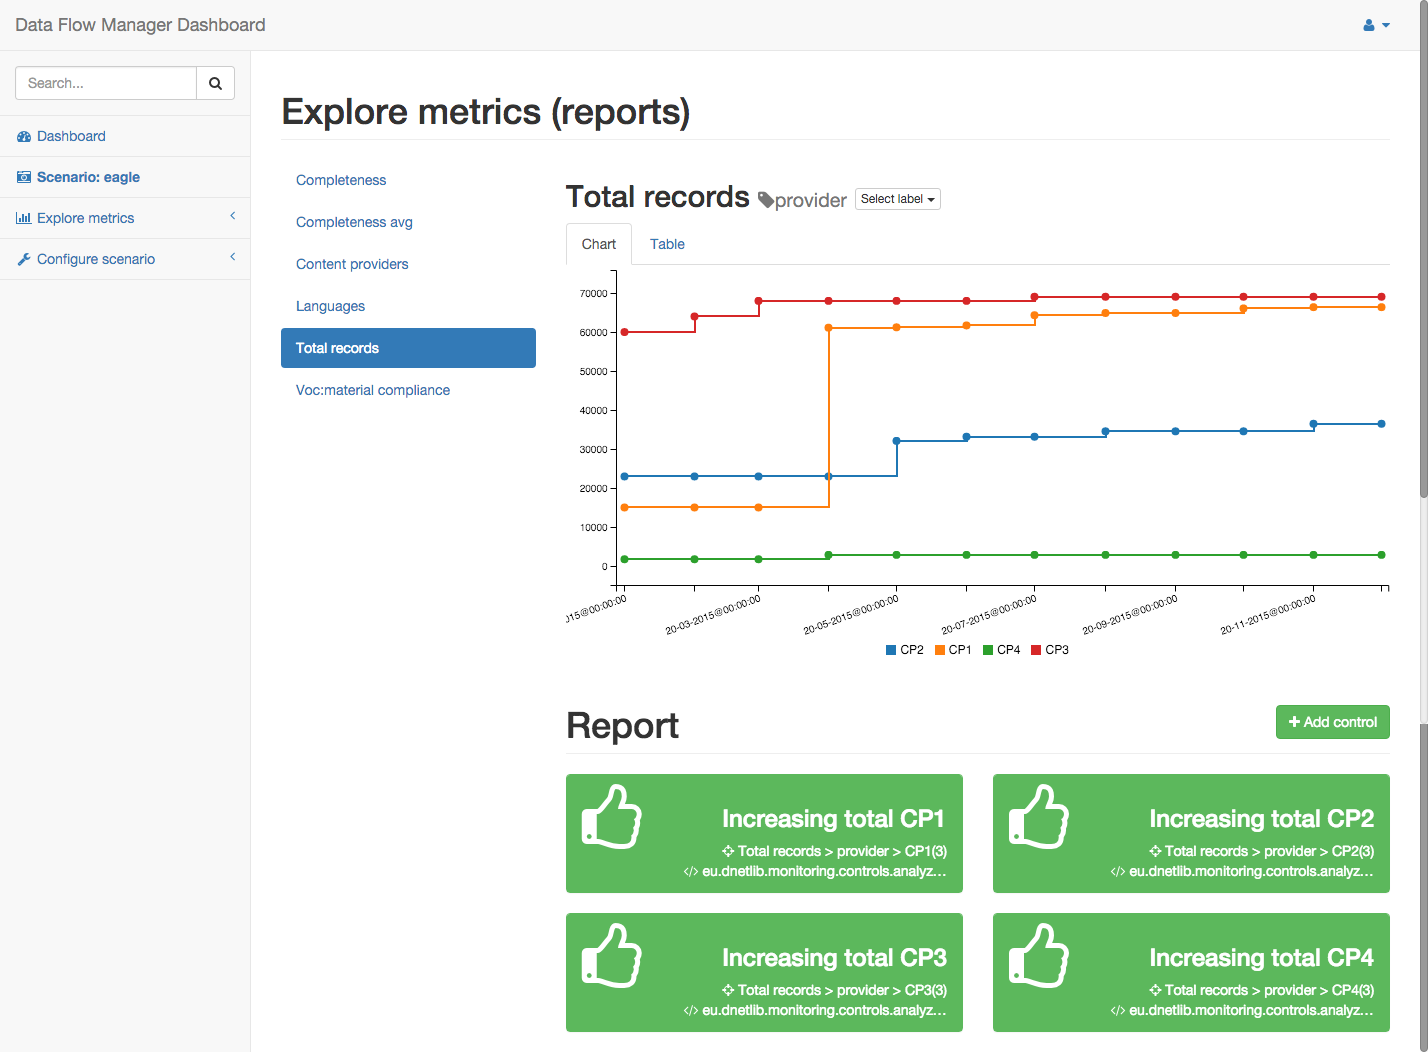
\includegraphics[width=\textwidth]{img/tot.png}
\caption{The trend of the metric ``Total records''.}
\label{fig:tot}
\end{figure}

\begin{figure}[H]
\centering
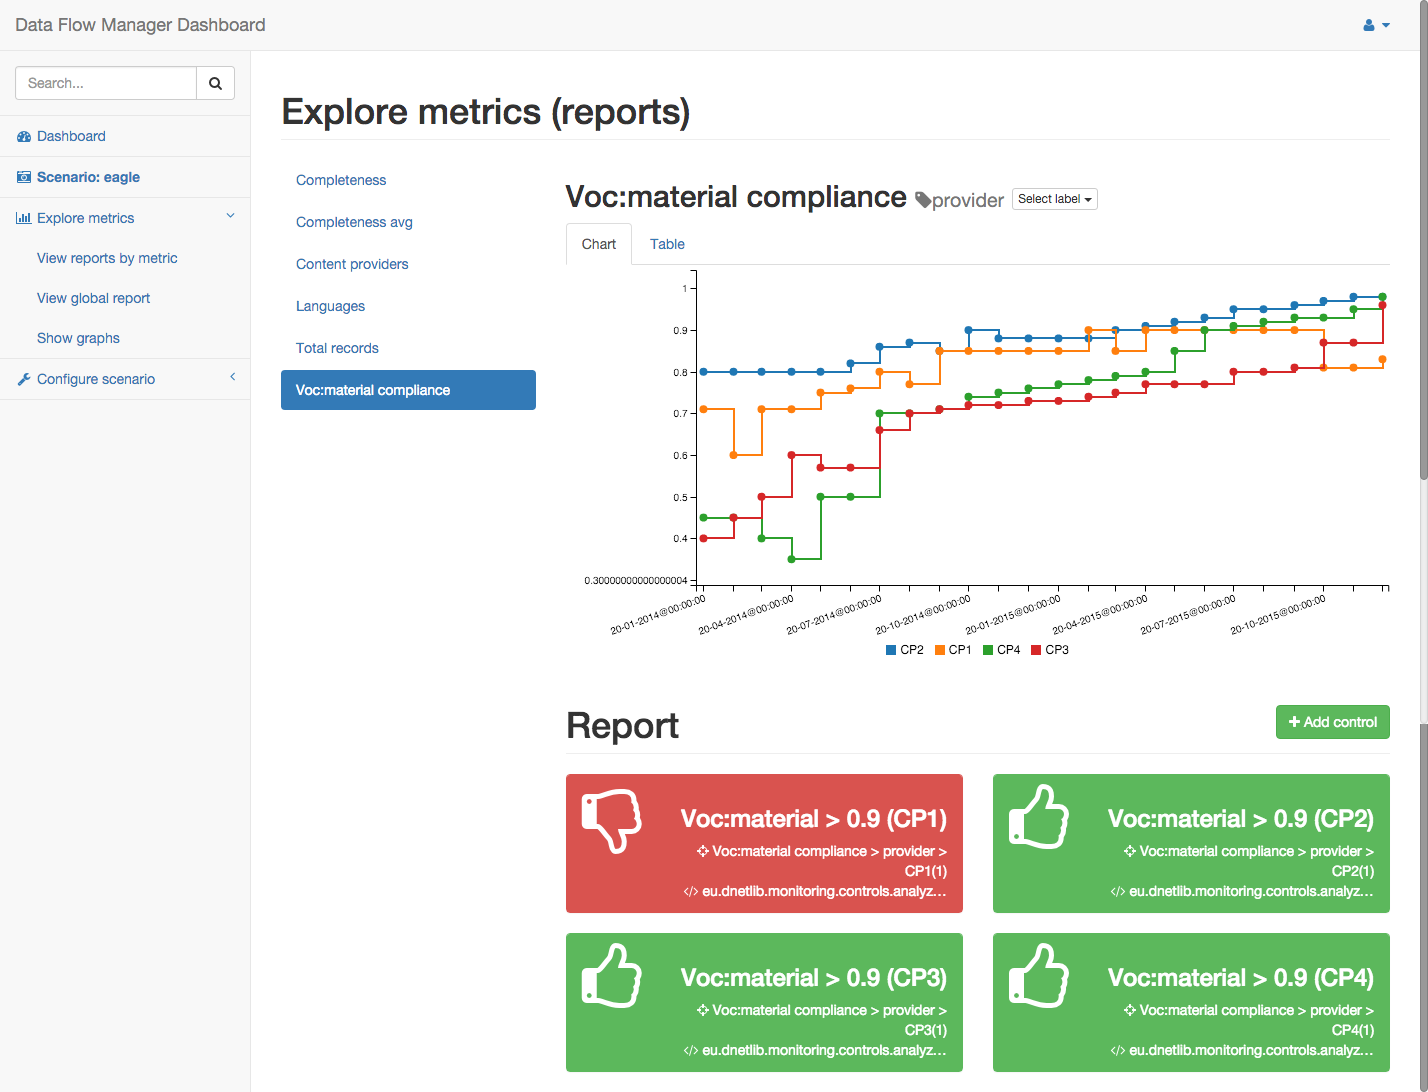
\includegraphics[width=\textwidth]{img/voc.png}
\caption{The trend of the metric ``Voc:material compliance''.}
\label{fig:voc}
\end{figure}

\begin{figure}[H]
\centering
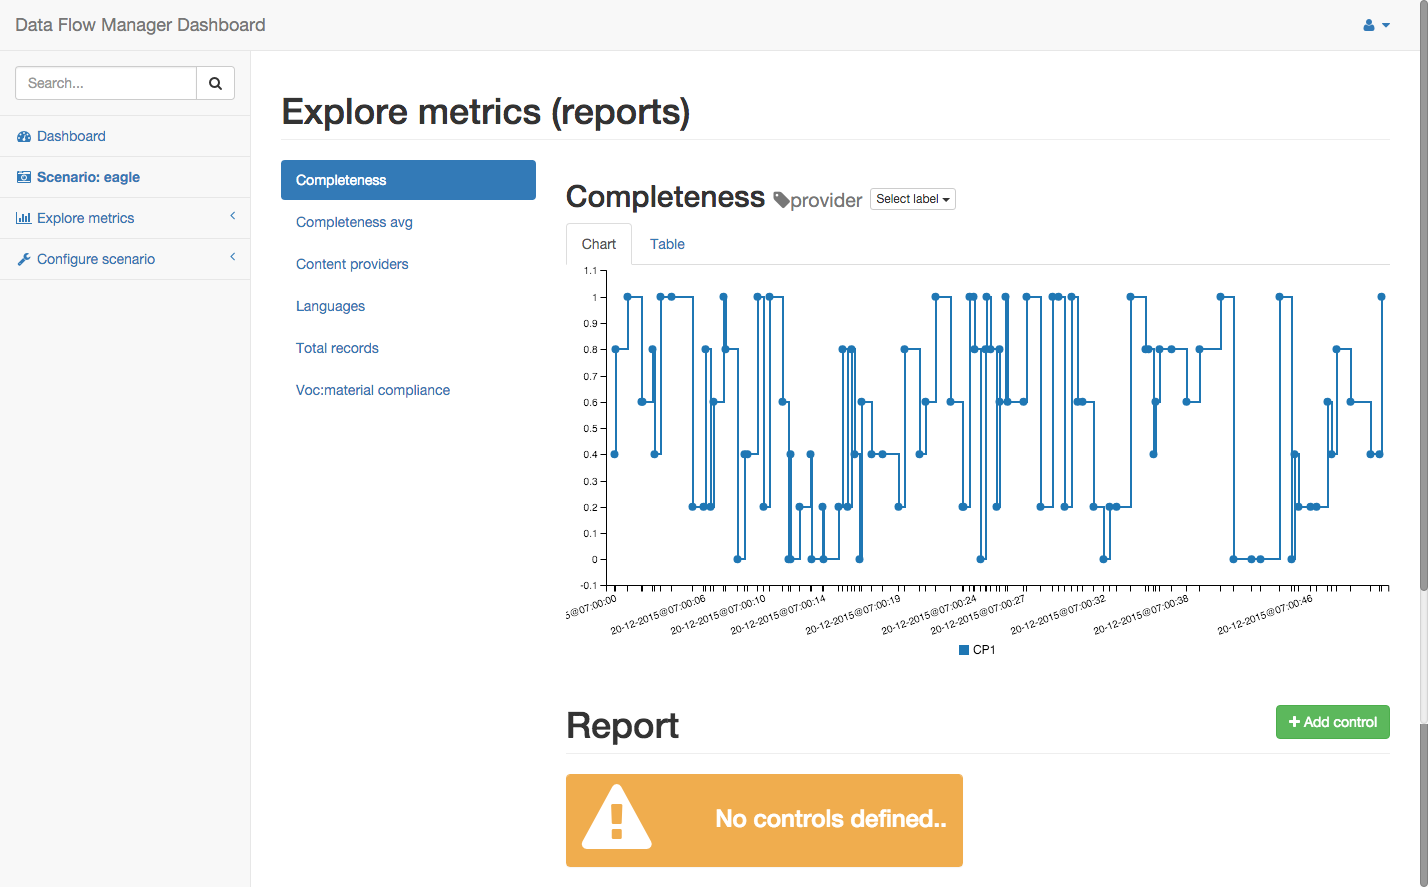
\includegraphics[width=\textwidth]{img/comp.png}
\caption{The trend of the metric ``Completeness''.}
\label{fig:comp}
\end{figure}

\begin{figure}[H]
\centering
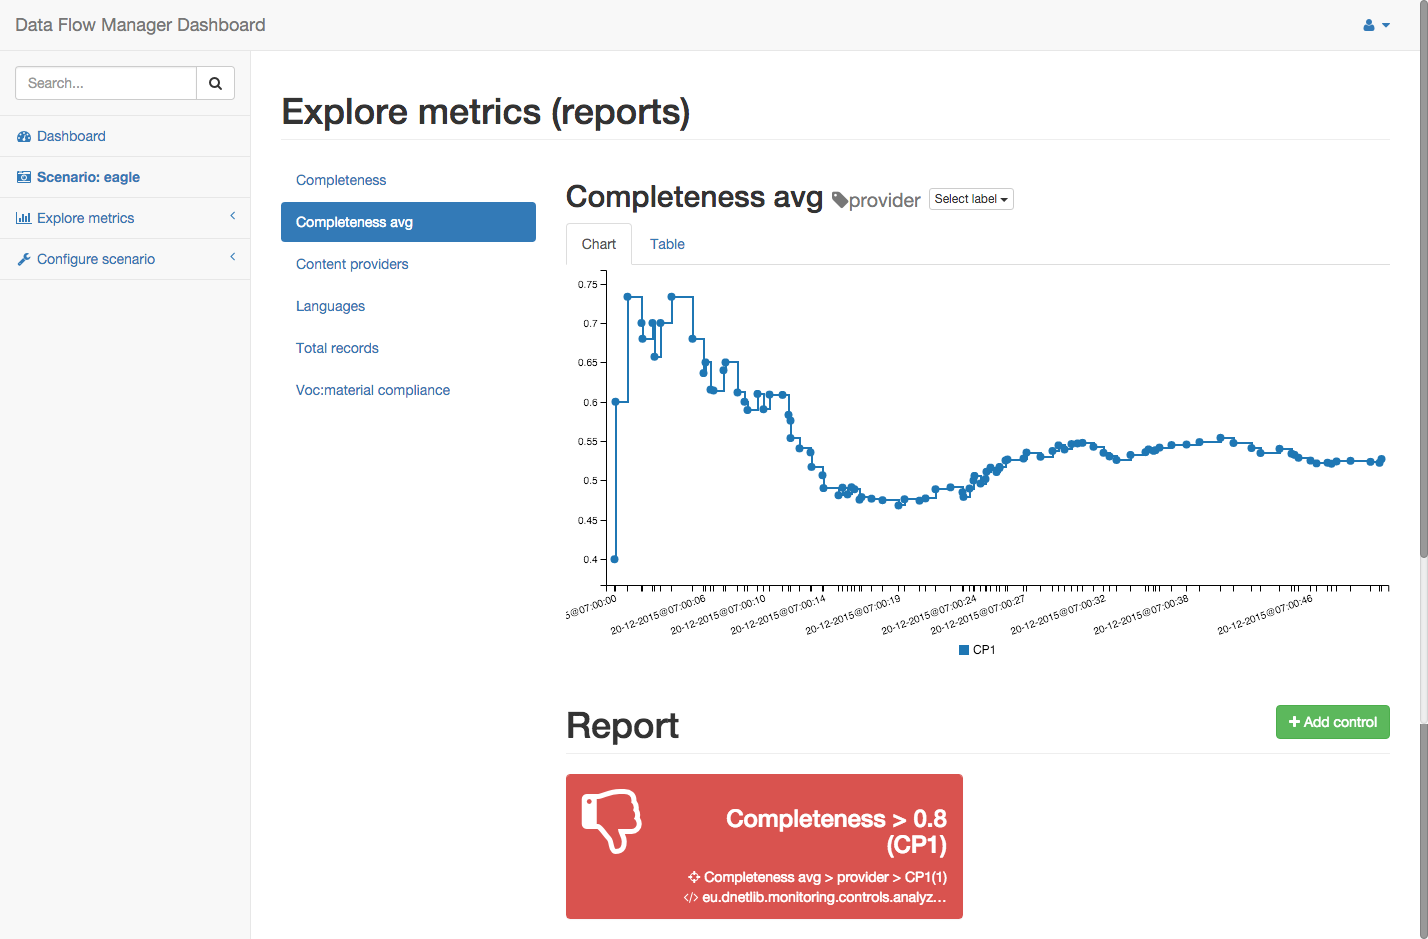
\includegraphics[width=\textwidth]{img/comp_ravg.png}
\caption{The ``rolling average'' of the metric ``Completeness''.}
\label{fig:ravg}
\end{figure}

\section*{Acknowledgements}
This work is partly funded by the EU EAGLE Best Practice Network project: Grant Agreement CIP 325122, call CIP-ICT-PSP-2012-6.


\bibliographystyle{sapauth-eng}
\bibliography{../../EAGLE}

\end{document}
